\documentclass[10pt]{beamer}

\usetheme{CambridgeUS}
\usepackage[english, russian]{babel}
\usepackage[utf8]{inputenc}
\usepackage{caption}
\usepackage{etoolbox}
\usepackage{multicol}
\usepackage{movie15}

\title[\href{https://goo.gl/NRgp8K}{https://goo.gl/NRgp8K} (Term 3)]{Длинная арифметика}
\author[Гусев Илья]{Гусев Илья}
\institute[МФТИ] 
{Московский физико-технический институт\\*}
\date{Москва, 2017}
\subject{Computer Science}

\begin{document}

\begin{frame}
  \titlepage
\end{frame}

\begin{frame}{Содержание}
\tableofcontents
\end{frame}

\section{Умножение}

\subsection{Умножение Карацубы}
\begin{frame}[fragile]{Умножение Карацубы}
\begin{center}
    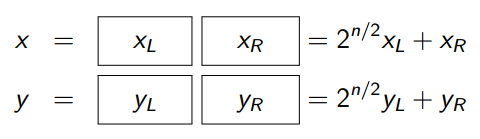
\includegraphics[width=7cm,height=2cm]{Term_3/Source/Pictures/karatsuba.png}\\
\end{center}
\textbf{Идея:}\\
$ x \cdot y = (2^\frac{n}{2} \cdot x_L + x_R)(2^\frac{n}{2} \cdot y_L + y_R) = 2^n \cdot x_L \cdot y_L + 2^\frac{n}{2}(x_L \cdot y_R + x_R \cdot y_L)+x_R \cdot y_R$\\
4 умножения \rightarrow $T(n) = 4 \cdot T(\frac{n}{2}) + O(n)$ \rightarrow $O(n^2)$
$ x \cdot y = 2^n \cdot x_L \cdot y_L + 2^\frac{n}{2}((x_L + x_R) \cdot (y_L + y_R) - x_R \cdot y_R - x_L \cdot y_L)+x_R \cdot y_R$\\
3 умножения \rightarrow $T(n) = 3 \cdot T(\frac{n}{2}) + O(n)$ \rightarrow $O(n^{log_2 3})$

\end{frame}

\subsection{БПФ}
\begin{frame}[fragile]{Дискретное преобразование Фурье}
ДПФ для $\vec x$: $\vec X = \hat A \vec x$, где $\hat A$:  $a_{N}^{mn} = e^ { -\frac{2\pi i}{N} mn}$\\
Идея ДПФ для полинома: полином в степени n $\Leftrightarrow$ значения в n+1 точках\\
ДПФ для полинома $A(x) = a_0 x^0 + a_1 x^1 + \ldots + a_{n-1} x^{n-1}$:  ${\rm DFT}(a_0, a_1, \ldots, a_{n-1}) = (y_0, y_1, \ldots, y_{n-1})  = (A(w_n^0), A(w_n^1), \ldots, A(w_n^{n-1}))$\\ 
$w_n^{k} = e^{ - i \frac{ 2 \pi k }{ n } }$\\
\end{frame}

\begin{frame}[fragile]{Дискретное преобразование Фурье}
Пример для $13 \Leftrightarrow 3 + x, 24 \Leftrightarrow 4 + 2x$:\\
\begin{bmatrix}
    1 & 1 & 1  & 1 \\
    1 & -i & -1 & i \\
    1 & -1 & 1 & -1\\
    1 & i & -1 & -i 
\end{bmatrix}
\times
\begin{bmatrix}
    3 \\
    1 \\
    0 \\
    0
\end{bmatrix}
=
\begin{bmatrix}
    4 \\
    3- i \\
    2 \\
    3 + i    
\end{bmatrix}
,
\begin{bmatrix}
    1 & 1 & 1  & 1 \\
    1 & -i & -1 & i \\
    1 & -1 & 1 & -1\\
    1 & i & -1 & -i 
\end{bmatrix}
\times
\begin{bmatrix}
    4 \\
    2 \\
    0 \\
    0
\end{bmatrix}
=
\begin{bmatrix}
    6 \\
    4- 2i \\
    2 \\
    4 + 2i    
\end{bmatrix}\\
\begin{bmatrix}
    4 & 3- i & 2 & 3 + i    
\end{bmatrix}
\times
\begin{bmatrix}
    6 \\
    4- 2i \\
    2 \\
    4 + 2i    
\end{bmatrix}
=
\begin{bmatrix}
    24 \\
    10 - 10i \\
    4 \\
    10 + 10i    
\end{bmatrix}\\
\frac{1}{4}
\times
\begin{bmatrix}
    1 & 1 & 1  & 1 \\
    1 & i & -1 & -i \\
    1 & -1 & 1 & -1\\
    1 & -i & -1 & i 
\end{bmatrix}
\times
\begin{bmatrix}
    24 \\
    10 - 10i \\
    4 \\
    10 + 10i    
\end{bmatrix}
=
\begin{bmatrix}
    12 \\
    10 \\
    2 \\
    0   
\end{bmatrix}\\
$12 + 10x + 2x^2 \Leftrightarrow 12 + 100 + 200 = 312$
\end{frame}


\begin{frame}[fragile]{Быстрое преобразование Фурье}
Идея БПФ: разделяй и властвуй:\\
$A_0(x) = a_0 x^0 + a_2 x^1 + \ldots + a_{n-2} x^{n/2-1}$\\
$A_1(x) = a_1 x^0 + a_3 x^1 + \ldots + a_{n-1} x^{n/2-1}$\\
$A(x) = A_0(x^2) + x A_1(x^2)$ \\
$y_k = y_k^0 + w_n^k y_k^1, ~~~~k = 0 \ldots n/2-1$\\
$y_{k+n/2} = y_k^0 - w_n^k y_k^1, ~~~~k = 0 \ldots n/2-1$\\
$y_{k+n/2} = A(w_n^{k+n/2}) = A_0(w_n^{2k+n}) + w_n^{k+n/2}A_1(w_n^{2k+n})= A_0(w_n^{2k}) - w_n^k A_1(w_n^{2k}) = y_k^0 - w_n^k y_k^1$\\
\end{frame}

\begin{frame}[fragile]{Быстрое преобразование Фурье}
Обратное - через обратную матрицу к $\hat A$\\
${\rm DFT} (A \times B) = {\rm DFT} (A) \times {\rm DFT} (B)$\\
$ A \times B = {\rm InverseDFT}( {\rm DFT} (A) \times {\rm DFT} (B) )$\\
Коэффициенты многочлена - числа в разрядах\\
Сложность: $O(n \cdot log(n))$\\
\end{frame}


\appendix
\section<presentation>*{\appendixname}
\subsection<presentation>*{Useful links}

\begin{frame}[allowframebreaks]
  \frametitle<presentation>{Полезные ссылки}
    
  \begin{thebibliography}{10}
{
  \beamertemplatebookbibitems
  
  \bibitem{E-maxx: FFT}
   \texttt{E-maxx: FFT}
  \newblock \href{http://e-maxx.ru/algo/fft\_multiply}{\texttt{http://e-maxx.ru/algo/fft\_multiply}}
  
  \bibitem{Wiki: DFT}
   \texttt{Wiki: DFT}
  \newblock \href{https://en.wikipedia.org/wiki/Discrete\_Fourie\_transform}{\texttt{https://en.wikipedia.org/wiki/Discrete\_Fourie\_transform}}
}
    
  \end{thebibliography}
\end{frame}

\end{document}


